\section{两阶段为什么值得分开}
\label{sec:why}

\subsection{资源画像的相反性}

把两阶段当成同一种工作来对待，是混部方案的默认假设；分离的全部合理性
都建立在「这个假设不成立」之上。所以先看它在哪不成立。

三篇独立工作给出同一判断。DistServe 指出 LLM 服务的延迟由两个指标定义：
首 token 时延（TTFT）对应 prefill 阶段，每输出 token 时延（TPOT）对应
decode 阶段\texttt{[c-profile]}。Sarathi-Serve 进一步说明两者的瓶颈不同
（见第 1 节引文）。Splitwise 的表述最直接：他们把 LLM 推理请求的
两个阶段\textbf{拆到不同的机器上}，理由是这样可以用「更贴合各阶段特性」
的硬件。

\subsection{差异如何限制混部}

两阶段放在同一张卡上时，必须共享同一套配置：同一个并行度、同一个
batch 上限、同一个显存配额。这对两阶段都是次优的。

\begin{itemize}[leftmargin=1.3em,itemsep=1.5pt,topsep=2pt]
  \item \textbf{并行度冲突。} prefill 偏好更大的张量并行以摊薄单次
        大矩阵乘的时延；decode 偏好更小的并行以降低通信占比。
  \item \textbf{batch 冲突。} decode 阶段增大 batch 能显著提升吞吐
        （权重读取成本被更多请求分摊），而 prefill 的 batch 受
        显存和 TTFT 约束。
  \item \textbf{显存冲突。} prefill 需要大块临时激活内存，
        decode 需要尽量多的 KV cache 空间。两者抢同一块显存。
\end{itemize}

分离的收益正来自解除这三处冲突。但要注意：\textbf{收益的大小取决于
两阶段的最优配置差多远}，而不是取决于分离这个动作本身。
小模型、短上下文、单卡可容纳全部权重与 KV 的场景下，两阶段的最优配置
可能很接近，此时分离的收益就很小，甚至为负\texttt{[c-formula]}。

\begin{figure*}[t]
  \centering
  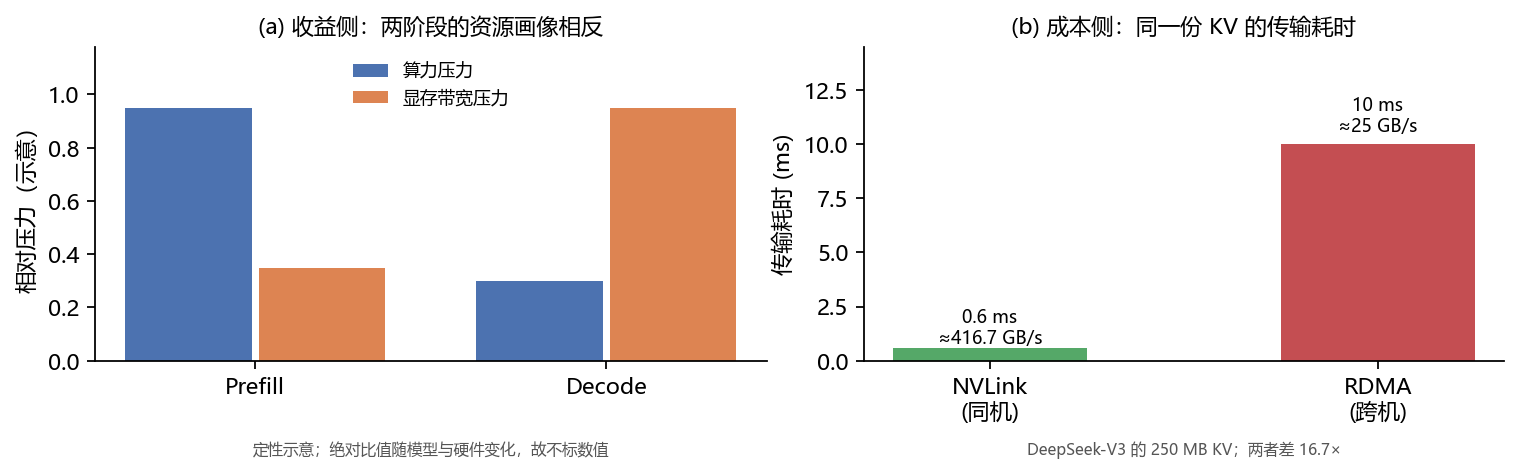
\includegraphics[width=0.92\textwidth]{figures/fig1_cost_benefit.png}
  \caption{分离的收支两侧。(a) 收益侧：prefill 与 decode 的资源画像相反，
  这是分离的唯一理由；此处为\textbf{定性示意}，不标具体数值，因为绝对
  比值随模型与硬件显著变化。(b) 成本侧：同一份 250\,MB KV cache 经
  NVLink 传输 0.6\,ms、经 RDMA 传输 10\,ms，相差 16.7 倍。
  两侧对照说明：分离是否划算，取决于收益能否盖过这个成本。}
  \label{fig:cost}
\end{figure*}
